\documentclass[11pt]{article}
\usepackage[margin=1in]{geometry}
\usepackage{booktabs}
\usepackage{graphicx}
\usepackage{amsmath}
\begin{document}
\section*{Pseudo-outcome weights along the sampling path}

Each stream uses the same loop. The reference window is source then target. The pool is half and half. The test set is target only. Every query rule runs twice from the same source-trained network: once with a flat weight, once with the per-row pseudo-outcome residual from a nuisance fit that scores pool rows as $T=1$. Training is five rounds of SGD, batch size 32, three epochs per round, hidden width 64. Seeds are 0 and 1. The band is the standard deviation across rules, not across seeds.

Digits: 8$\times$8 digits, pixels in $[0,1]$, target rolled two columns. Pen digits: 16 stroke coordinates in $[0,1]$, target $x$-coordinates $+0.25$. Satimage: 36 standardized bands, first 9 bands of the target $+1.25$.

\begin{figure}[t]
\centering
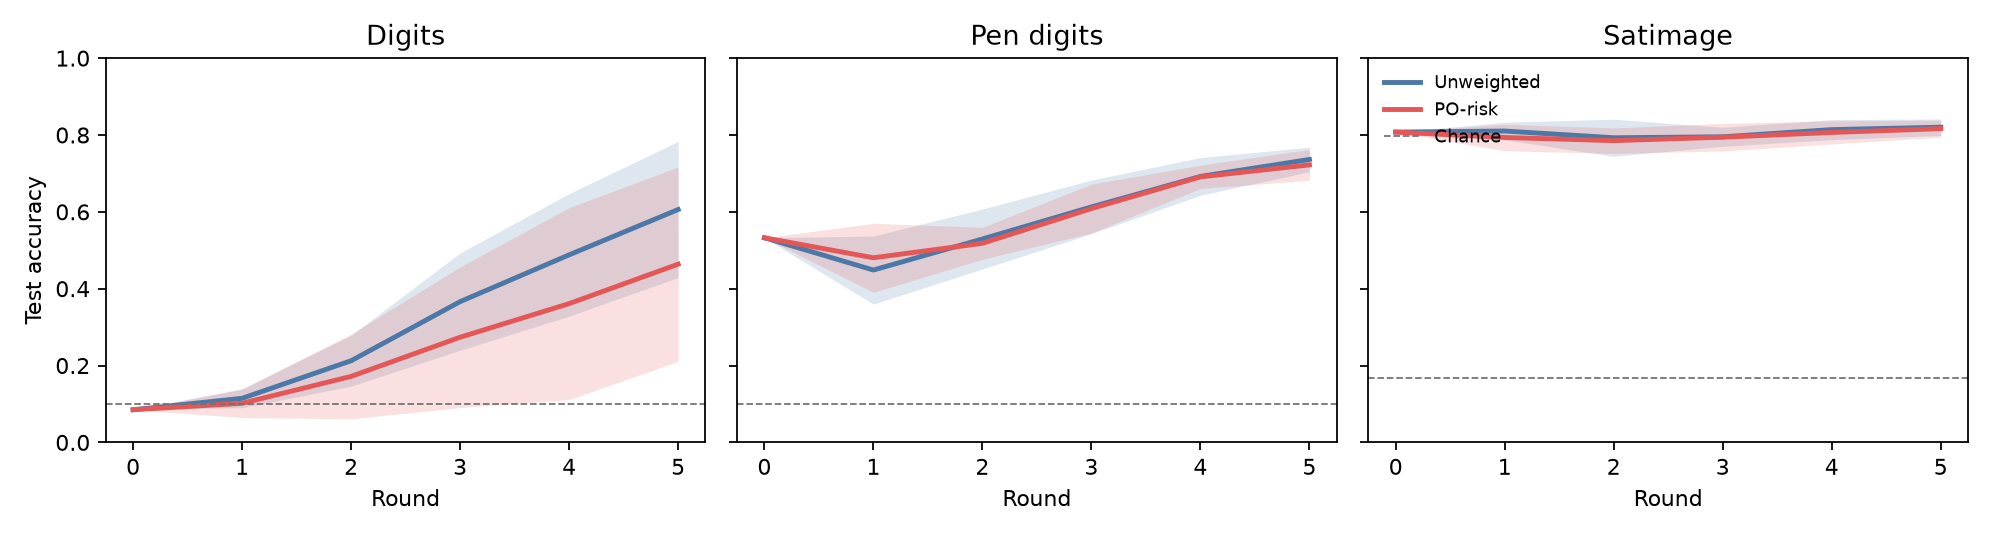
\includegraphics[width=\textwidth]{mean_paths.png}
\caption{Mean test accuracy by round. Round 0 is the source model. The dashed line is chance.}
\label{fig:po-weight-paths}
\end{figure}

\begin{table}[t]
\centering
\caption{Mean test accuracy over query rules, two seeds. k-center is omitted because it repeats core-set. The pool is half target rows. Chance is $1/C$.}
\label{tab:po-weight-summary}
\begin{tabular}{lrrrrrrr}
\toprule
Dataset & $C$ & Unweighted & PO-risk & AUC plain & AUC PO & Share plain & Share PO \\
\midrule
Digits & 10 & 0.606 & 0.464 & 0.305 & 0.237 & 0.433 & 0.338 \\
Pen digits & 10 & 0.736 & 0.722 & 0.583 & 0.585 & 0.502 & 0.392 \\
Satimage & 6 & 0.820 & 0.816 & 0.805 & 0.798 & 0.527 & 0.449 \\
\bottomrule
\end{tabular}
\end{table}

\begin{table}[t]
\centering
\caption{Final accuracy with the pseudo-outcome weight minus the unweighted run, in percentage points. Positive means the weight finished higher.}
\label{tab:po-weight-delta}
\begin{tabular}{lrrr}
\toprule
Rule & Digits & Pen digits & Satimage \\
\midrule
\texttt{cluster\_margin} & +7.0 & +3.5 & +0.0 \\
\texttt{margin} & +5.5 & +7.3 & -2.7 \\
\texttt{baseline} & -5.5 & +6.2 & +4.2 \\
\texttt{adversarial\_bim} & +10.5 & -5.5 & -1.0 \\
\texttt{kmeans} & +0.0 & +0.5 & +0.0 \\
\texttt{margin\_dropout} & +2.2 & +1.5 & -3.5 \\
\texttt{adversarial\_deepfool} & +1.0 & -2.3 & -1.5 \\
\texttt{albl} & -9.5 & +4.0 & +2.2 \\
\texttt{random} & -10.5 & +2.0 & -1.2 \\
\texttt{batch\_bald} & -12.0 & -6.0 & -3.7 \\
\texttt{bald} & -14.5 & -5.5 & -2.8 \\
\texttt{badge} & -16.8 & -9.0 & +0.2 \\
\texttt{entropy} & -29.3 & -1.5 & +4.7 \\
\texttt{coreset} & -29.2 & -15.5 & +0.7 \\
\texttt{least\_confidence} & -42.2 & -1.0 & -1.0 \\
\texttt{entropy\_dropout} & -43.2 & -2.3 & -0.5 \\
\texttt{least\_confidence\_dropout} & -55.2 & -0.5 & -0.7 \\
\midrule
Mean & -14.2 & -1.4 & -0.4 \\
\bottomrule
\end{tabular}
\end{table}

On digits the pseudo-outcome weight lowers the mean final accuracy from 0.606 to 0.464. On pen digits the pseudo-outcome weight lowers the mean final accuracy from 0.736 to 0.722. On satimage the two mean final accuracies meet (0.820 unweighted, 0.816 weighted). On satimage the source model already scores 0.807 on the target, so the later rounds have little accuracy left to gain.

\end{document}
